\documentclass{IOS-Book-Article}

% gb4e is buggy
\makeatletter
\def\new@fontshape{}
\makeatother

\usepackage[utf8]{inputenc}
\usepackage{amsmath}
\usepackage{amssymb}
\usepackage{amsthm}
\usepackage{mathptmx}
% \usepackage{caption} % for \figsentence
\usepackage{subcaption} % for subfigure
\usepackage{graphicx}
\usepackage{tikz}
\usepackage{tikz-qtree}
\usepackage{syntax} % for grammar environment
\usetikzlibrary{arrows.meta,positioning,patterns}
\usepackage{hyperref} % for urls
\usepackage{gb4e}

\newcommand{\figsentence}[1]{\\{\sffamily{}#1}}

\tikzset{
	x/.style={{Rays[]}},
	-x/.style={-{Rays[]}},
	xx/.style={Rays[]}-{Rays[]},
	box/.style={draw,rectangle,align=center},
	assumed/.style={pattern=crosshatch dots,pattern color=gray},
	every new ->/.style={shorten >=1pt}
}

\begin{document}

	\begin{frontmatter}

		\title{Arguments that can be understood \\by humans and by computers}

		\author{Jelmer VAN DER LINDE, Bart VERHEIJ}

		\address{Artificial Intelligence, University of Groningen}

		\begin{abstract}
	Good argumentation technology requires that humans and computers understand each other's arguments.
	But notwithstanding significant research progress, meeting this requirement remains hard to realize. Formal models underlying argumentation software can be hard to interpret for people (cf. the intricacies of research on argumentation formalisms), and computers can have a hard time understanding natural language arguments made by humans (cf. the complexity of argument mining research).

	In this paper, we develop a restricted argumentation model that is equally understandable for humans and for computers. Concretely, we realize the model in a natural language format and in a formal argument format, visualized as diagrams. It is our strategy to work from the ground up: starting from simple structures gradually moving to more complex structures. We choose this strategy in order to optimize the tractability of successes and resolvability of hurdles. In the restricted argumentation model proposed in this paper we focus on arguments for and against elementary conclusions, and on the rules (warrants, generalizations) underlying them. For evaluating our proposal, we discuss syllogisms and Toulmin arguments.

	The core model of argumentation that we discuss is relevant for formal research on argumentation, since it focuses on argument structure that can be expressed in a computationally understandable natural language form; the core is relevant for argument mining research, since it presents a restricted natural language setting of which the formal structure is computationally understandable.

		\end{abstract}

		\begin{keyword}
		Argument diagrams, argument mining, natural language processing, Toulmin
		\end{keyword}

	\end{frontmatter}

\section{Introduction}
Human communicate and share their knowledge and understanding of their world by arguing with each other. If computers and humans could have a shared argumentation process, they could understand each other better.

\paragraph{Current}
The structure of arguments has been analysed since Aristotle, trying to identify, understand and formalize the workings and structure of arguments which we so effortlessly use every day.

Argumentation, from the perspective or Artificial Intelligence, has focussed mainly on the structure and evaluation of arguments: is this claim true, given these arguments either in favour or opposed it~\cite{vanEemerenEtal2014ch11}.

\paragraph{Non-formal and formal argumentation theory}
Arguments occur in every form of human communication, in dialogue, monologue, explicitly written or almost subliminally implied while conveying information in any form. What all these forms do share is the concept of claims that are made, and that are attacked or supported by other claims, either in the forms of reasoning, or examples, or counter-examples. Formalising this structure is challenging, and the various approaches vary in their focus and formalism\cite{vanEemerenEtal2014,vanEemerenVerheij2017}. For example, Aristotle's syllogism created the dichotomy between minor and major premises, where the major premise serves as a generalized case (i.e. birds can fly) and the minor premise argues that this generalization is applicable (i.e. Tweety is a bird), and thus the conclusion is valid (i.e. Tweety can fly.).

\paragraph{Toulmin's model}
Toulmin\cite{toulmin1958} in a sense continues this work, formalising not only the minor and major premise and conclusion (which roughly translate to his datum, warrant and conclusion) but also dictates which additional elements should be present in a well formulated argument, and what outside of syllogisms the role of a warrant should be: each inference, i.e. each claim supporting a conclusion should be defensible by a warrant, a generalization why this conclusion may be concluded given the supporting datum. This generalization in turn should also be based in evidence, or in logic; it should be supported by a backing. Furthermore, the generalization almost always comes with a qualifier: how certain it is that the generalization is applicable in this situation, which range includes an analytical `all' in claims such as `all penguins are birds' to a statistical `most' in `most swans are white'. And last but not least the option for attack of a conclusion (i.e. a counter-argument) becomes part of the argument, uniting both support and attack in the same model. Toulmin's model of an argument dictates what may elements may be expected in an argument, either explicitly stated or answerable when asked. The elements described in this model form the basis for more formal approaches\cite{verheij2009}.

\paragraph{Walton argument schemas}
Walton started with documenting common structures~\cite{waltonReedMacagno2008} used in argumentation, marking their elements. In a sense, this these schemas extend the formalisation of Toulmin's warrant, and extend the idea of Toulmin's model to more specific arguments in general: Walton's argument schemas also propose critical questions. Walton, and many others, defined such schemas based on the arguments they encountered. Consequently, there is no complete set of all schemas. The schemas are now often used for annotating the relation between parts of arguments, either automatically or using manual annotation.

\paragraph{Argument mining}
With the availability of large corpora of written and annotated text\cite{lawrenceReed2015} and advances in natural language processing, as well as the drive to automate the extraction of computer-understandable information, the challenge of argument mining has thrived. \cite{moens2017,peldszus2013argument,lippi2016argumentation,mochales2011argumentation}

This extraction process of information is the practise of discourse analysis. Approaches to discourse analysis usually aim at identifying various different types of discourse relations. However, we are only interested in a subset of such relations, namely those relevant for argumentation structure parsing. This smaller task is often referred to as Argument Mining~\cite{stabGurevych2017} and this task generally consists consists of multiple subtasks~\cite{lippi2016argumentation}:

\paragraph{Identification} The parts of text that are argumentative –- that may contain arguments -- need to be identified: In many texts only certain sentences or paragraphs of the text are argumentative; the rest may be informative, for example providing context. In it's essence this is a binary classification task. Some approaches combine this task with the next and directly detect and classify the argument components~\cite{stabGurevych2017}. In this case the classifier is also tasked with detecting the type of component (e.g. conclusion, minor or major premise, etcetera depending on the structural model used.)

\paragraph{Segmentation} The identified parts need to be split into segments -- the task of component boundary detection -- where each segment may be a component in the final argument representation. Assuming that in a text about a court case the paragraphs containing the ruling and the reasoning behind it are identified, then this step splits that part into components (called argumentative discourse units~\cite{cohen1987} or elementary discourse units~\cite{saintDizier2012}) that can then be identified as the conclusion, premises, etc. This, again, is a classification task. This is implemented as a data-driven search for cue phrases (i.e. the words `because', `unless', but also words, word phrases and punctuation that are less explicit, or a complete analysis of the semantic structure) that indicate relations between text spans~\cite{mochales2011argumentation,saintDizier2012,lawrenceReed2015,stabGurevych2017}.

\paragraph{Prediction} The relations between the identified components need to be predicted. In this task the components are connected to each other to form the structure of the argument. This is the most challenging task as it requires insight in the meaning of a component to determine whether a premise component supports a certain claim component or whether it is related to another claim component. Some approaches also approach this as a binary classification task, testing each of the claim components in a certain defined order~\cite{cohen1987}. Others have a set of hand-coded rules that function as heuristic~\cite{saintDizier2012}. Another approach is to create a model that can determine the likeliness that two components are related and construct multiple scenarios to finally select the best overall scenario. Often knowledge about the domain is used to help in this task. For example, for some texts, such as procedures or didactic text, it can be assumed that a claim is always followed by one or more premises supporting that claim. In juristic texts certain marker words may signal the relations between components.

Most approaches are based on text which has been annotated using RST and a predefined set of schemas. The rules used in the three subtasks are, either by hand or automatically, derived from these previously annotated texts to create a model which can apply the same annotation to new texts.

\paragraph{Argumentation software}
Argumentation in Artificial Intelligence results in argumentation software, programs that often focus on understanding and teaching argumentation\cite{kirschnerEtal2003,scheuerEtal2010,noroozi2012argumentation}, as well as serve as a proof-of-concept of various formalisms,\cite{verheij2007}.

\paragraph{Our idea}
Our approach to understanding argumentative texts is based on a schematic representation of arguments in the form of boxes for claims and arrows for the support and attack relations between these claims \cite{peldszus2013argument,verheij2007}. Based on this schematic representation and its elements we define a grammar for a natural language on how to formulate these argumentative structures. Our human argumentative structure language (HASL) allows us to write argumentative text which can be directly interpreted as an argument diagram.

\paragraph{Goals}
Support and attack relations between arguments, warranted support in the form of general rules that support the step from premise to conclusion (i.e. major premise in syllogism). The ability to combine sentences to counter the need to restate premises (i.e. allow recursion). Anaphora resolution to avoid the need to restate the subjects. Enthymeme resolution to avoid the need to state many premises at all. 

\paragraph{Results}
For each of the basic building blocks for formal argumentation we define how these occur in our language, and how they can be differentiated form each other.

We implement these building blocks and their grammars into a larger grammar which allows us to create argumentative texts of multiple sentences. This language, the human argument structure language, or HASL for short, is explored in two variants.

We then test our implementation using the following examples:
\begin{exe}
	\ex\label{ex:socrates} Socrates is mortal because he is a man and men are mortal.
	\ex\label{ex:tweety} Tweety can fly because Tweety is a bird and birds can fly but Tweety is a penguin and penguins can not fly.
	\ex\label{ex:light} The object is red because the object appears red to me but it is illuminated by a red light.~\cite{pollock1987}
	\ex\label{ex:toulmin} Harry is a British subject because Harry was born in Bermuda and a man born in Bermuda is a British subject because of the following statutes and legal provisions but Harry has become a naturalized American.~\cite{toulmin1958}
\end{exe}

\paragraph{HASL}
Our experimental human argument structure language (HASL) implements a grammar for combining the building blocks by restating premises in multiple sentences. Each of the building blocks yields its own partial argument structure, which are merged at the sentence level to form the complete argument. This implementation does a complete parse of the premises themselves as well to differentiate between major and minor premises.

The grammar allows for nested argument structures: A premise that occurs on the right side of `because' can itself be the conclusion of a different part of the argument in the same sentence.

We implement a form of enthymeme resolution. Enthymemes, the occurrence of premises that are part of an argument but are not explicitly stated, occur often in natural language \cite{walton2005,reedRowe2004}. By filling in these missing premises in our argument graph we can make the right support or attack connections between premises, also when the targeted premise is not explicitly stated. We do this by treating building block around the attack and support relations as small syllogisms, and reconstruct the missing minor or major premise. The parsing of premises themselves, which is a part of HASL/1, provides the information necessary for the reconstruction.

We also implement pronominal anaphora resolution \cite{hobbs1978}. In HASL/1 premises that are the same are merged into a premise in our argument structure, and in HASL/1 we determine whether two premises are the same by comparing their text. When this text contains references to other parts of the argument, for example if the premise is `he has wings', we should also check whether `he' refers to the same object. Otherwise, premises that look the same but don't exactly mean the same are merged. Anaphora resolution helps us check this. By implementing this as part of the premise parser the reconstruction step of the enthymeme resolution can also profit from it.

\paragraph{Relevance}
HASL implements a form of argument mining, but ignores the difficult steps of being able to parse all of the English language. This allows us to explore what a complete understanding of the argumentative text entails, which argument mining is not yet able to explore \cite{stabGurevych2017}.

The implementations of HASL presented here can be used to gain a better understanding of complicated arguments, where there are many premises that interact with each other. Anaphora and enthymeme resolution help with further understanding of the argument.

The language of HASL itself can be used to a new type of interface to the reasoning process of computer programs, allowing for the explanation of the reasoning behind a conclusion, or even for interactive partaking.

\section{HASL}
HASL is an implementation of the language which focusses on supporting all elements of the argument structure. Combining sentences (or structures) in to larger arguments is done by repeating the premise, not unlike repeating a variable in first-order logic.

\paragraph{Parser} Sentences are tokenized and to each of the tokens a part-of-speech tag (pos-tag) is assigned using spaCy\cite{spacy2}. The tokens are then parsed into argument structures using an Earley parser and the grammar described in this section.

\paragraph{Argument structure} The partial and final argument structures are represented as a graph with nodes and edges, or claims and relations, with a few notable differences: First, a relation can have multiple claims as source to model Cooperative supporting relations between claims (\autoref{fig:linked}). Second, a relation can target another relation. This is needed to encode the warranted support relation (\autoref{fig:warrantedsupport}).

\paragraph{Merging arguments} At the end of every grammar rule the matched structures are merged. For rules that combine a few words into an \emph{object} this merely involves combining the spans of text into a single span that encompasses both (i.e. `the' + `man' becomes `the man') but when combining sentences the argument structures need to be merged. During this merge claims that were repeated in the text are merged into a single node in the argument graph.

\begin{enumerate}
    \item All claims from both arguments to be merged are added to the list as a pair consisting of the claims id and the claim itself.
    \item Each claim that occurs multiple times in the list is then replaced with the first occurrence.
    \item The list is used to replace all occurrences of the replaced claims with their replacement in the relations.
    \item The resulting set of unique claims and up-to-date relations is used to create a new argument, the result which is yielded after finishing the grammar rule.
\end{enumerate}

\subsection{Pros and cons}
Support relations between claims (\autoref{fig:support}) are the basis of argumentation: These indicate a reason to come to a certain conclusion.

Attack relations (\autoref{fig:attack}) indicate that a claim is, or has at some moment in the argumentative text been, disputed. The attack can be mutual: two claims exclude the possibility of each other, for example Socrates being mortal and Socrates being immortal. We draw these as two relations collapsed into one bidirectional one, shown in \autoref{fig:mutual}.

\begin{figure}[ht!]
    \centering
    \begin{subfigure}[b]{0.3\textwidth}
        \centering
        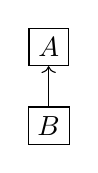
\begin{tikzpicture}
            \node[box] (con) at (0,0) {$A$};
            \node[box] (pre) at (0, -1) {$B$};
            \draw[->] (pre) to (con);
        \end{tikzpicture}
        \figsentence{$A$ because $B$.}
        \caption{Support}
        \label{fig:support}
    \end{subfigure}
    \begin{subfigure}[b]{0.3\textwidth}
        \centering
        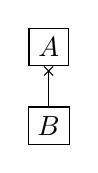
\begin{tikzpicture}
            \node[box] (con) at (0,0) {$A$};
            \node[box] (att) at (0, -1) {$B$};
            \draw[-x] (att) to (con);
        \end{tikzpicture}
        \figsentence{$A$ but $B$.}
        \caption{Attack}
        \label{fig:attack}
    \end{subfigure}
    \begin{subfigure}[b]{0.3\textwidth}
        \centering
        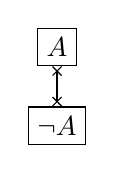
\begin{tikzpicture}
            \node[box] (con) at (0,0) {$A$};
            \node[box] (att) at (0, -1) {$\neg A$};
            \draw[xx] (att) to (con);
        \end{tikzpicture}
        \figsentence{$A$. $\neg A$.}
        \caption{Mutual attack}
        \label{fig:mutual}
    \end{subfigure}
    \caption{Pros and Cons}
    \label{fig:proscons}
\end{figure}

\paragraph{Grammar} We start with describing the grammar for the basic support and attack relations (Figures~\ref{fig:support} and~\ref{fig:attack}).

\begin{grammar}
<argument> ::= <claim> `because' <minor-claim> % *> a <~ b

<argument> ::= <claim> `but' <minor-claim> % *> a *~ b
\end{grammar}

\noindent After parsing the rule in a text the argument structure is formed. If we use $a$ and $b$ to denote the text that matched \texttt{<claim>} and \texttt{<minor-claim>} we can describe the argument yielded by matching the first rule as follows: It consists of two claims, conclusion $a$ and premise $b$, and a relation $b$ supports $a$ (\autoref{fig:support}).

Attacks (\autoref{fig:attack}) are parsed in a similar way, but with a different type of relation. Mutual attacks (\autoref{fig:mutual}) are written by writing two separate attack statements:

\begin{exe}
    \ex\label{ex:mutualsoc} Socrates is mortal but Socrates is immortal. Socrates is immortal but Socrates is mortal.
\end{exe}


\paragraph{Major and minor claims}
We make the distinction between minor and major claims: minor claims are statements about someone or something particular, e.g. Tweety, Socrates, and `the object' in our examples. Major claims are claims of a more general or generative nature: they are more rule-like and express expectations, for example that birds can fly or that men are mortal.

Minor and major claims are recognized in HASL using the following grammar rules. We use \texttt{<x>} with lower case $x$ to refer to other grammar rules, \texttt{<X>} with upper case $X$ to denote a token that matches one of the part-of-speech tags from \autoref{table:postags}, and \texttt{`x'} to indicate that the token is just the string `x'. Segments between square brackets are optional.

\begin{table}
    \begin{tabular}{lll}
        Tag & Description & Example \\
        \hline
        NN  & noun, singular & bird \\
        NNS & noun, plural & birds \\
        NNP & noun, proper singular & Socrates \\
        MD  & verb, modal auxiliary & can \\
        VBZ & verb, 3rd person singular present & is \\
        VBP & verb, non-3rd person singular present & are \\
        VBN & verb, past particle & illuminated \\
        DT  & determiner & the, a \\
        JJ  & adjective & red \\
        IN  & preposition & in, on, by \\
        RB  & adverb & not
    \end{tabular}
    \caption{Part-of-speech tags used in HASL, part of the Penn Treebank tag set.}
    \label{table:postags}
\end{table}

\begin{enumerate}
    \item `Tweety is a bird and `Socrates is not a man'
    \begin{grammar}
        <minor-claim> ::= <instance> <VBZ> [<RB>] <object>
    \end{grammar}
    \item `Tweety can fly'
    \begin{grammar}
        <minor-claim> ::= <instance> <MD> [<RB>] <VB>
    \end{grammar}

    \item `A man is mortal'
    \begin{grammar}
        <major-claim> ::= <prototype-sg> <VBZ> [<RB>] <object>
    \end{grammar}
    \item `A bird can fly'
    \begin{grammar}
        <major-claim> ::= <prototype-sg> <MD> [<RB>] <VB>
    \end{grammar}
    \item Men are mortal
    \begin{grammar}
        <major-claim> ::= <prototype-pl> <VBP> [<RB>] <object>
    \end{grammar}
    \item Birds can fly
    \begin{grammar}
        <major-claim> ::= <prototype-pl> <MD> [<RB>] <VB>
    \end{grammar}
\end{enumerate}

\noindent These rules are supported by definitions for \texttt{instance}, \texttt{object} and the singular and plural versions of \texttt{prototype}. These are defined in their own rules to make the major and minor claim rules more general. Effectively, minor claims begin with \texttt{instance}, major claims with \texttt{prototype}.

Objects are often the objects of sentences, although the rule is also reused for the parsing of prepositional phrases:

\begin{enumerate}
    \item `wings' in `Tweety has wings'
    \begin{grammar}
        <object> ::= <NN> \alt <NNS>
    \end{grammar}

    \item `red' in `the object is red'
    \begin{grammar}
        <object> ::= <JJ>
    \end{grammar}

    \item `the object' or `an object'
    \begin{grammar}
        <object> ::= <DT> <NN>
    \end{grammar}

    \item `the red light'
    \begin{grammar}
        <object> ::= <DT> <JJ> <NN>
    \end{grammar}

    \item `born in Bermuda' or `illuminated by a red light' for `the light is …'
    \begin{grammar}
        <object> ::= <vbn>

        <vbn> ::= <VBN>
        \alt <VBN> <preposition-phrase>

        <preposition-phrase> ::= <IN> <NNP>
        \alt <IN> <object>
    \end{grammar}
\end{enumerate}

\noindent Instances are names, nouns which are preceded by a definite determiner (e.g. `the', `this') and pronouns referring to them such as `he' and `it'.

\begin{grammar}
<instance> ::= <NNP>
\alt <PRP>
\alt <definite-dt> <NN>
\alt <definite-dt> <NNP>

<definite-dt> ::= `the' | `this'
\end{grammar}

\noindent Prototypes are the indefinite variant of these. Since major premises both often occur as singular and as plural premises we add grammar rules for both. For minor premises we have only added rules for the singular form.

\begin{grammar}
<prototype-sg> ::= <indefinite-dt> <NN> [<vbn>]

<prototype-pl> ::= <NNS> [<vbn>]

<indefinite-dt> ::= `a'
\end{grammar}

\paragraph{Sentences} Finally, an argumentative text in HASL's language consists of one or more sentences which combine the argument structures into a single argument diagram. Effectively a sentence is an argument ending with a period, and \texttt{sentences} is the top-most element of the parse tree.

\begin{grammar}
<sentences> ::= <sentences> <sentence>
    \alt <sentence>

<sentence> ::= <argument> `.'
\end{grammar}

\subsection{Conjunctions}

\begin{figure}[ht!]
    \centering
    \begin{subfigure}[b]{0.3\textwidth}
        \centering
        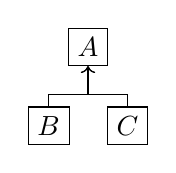
\begin{tikzpicture}
            \node[box] (con) at (0,0) {$A$};
            \node[box] (per1) at (-.5,-1) {$B$};
            \node[box] (per2) at (.5,-1) {$C$};
            \draw[->] (per1) -- ++(0,.4) -| (con);
            \draw[->] (per2) -- ++(0,.4) -| (con);
        \end{tikzpicture}
        \figsentence{$A$ because $B$ and $C$.}
        \caption{Cooperative support}
        \label{fig:linked}
    \end{subfigure}
    \begin{subfigure}[b]{0.3\textwidth}
        \centering
        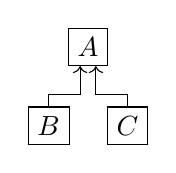
\begin{tikzpicture}
            \node[box] (con) at (0,0) {$A$};
            \node[box] (per1) at (-.5,-1) {$B$};
            \node[box] (per2) at (.5,-1) {$C$};
            \draw[->] (per1) -- ++(0,.4) -| ([xshift=-0.1cm]con.south);
            \draw[->] (per2) -- ++(0,.4) -| ([xshift=0.1cm]con.south);
        \end{tikzpicture}
        \figsentence{$A$ because $B$ and because $C$.}
        \caption{Independent support}
        \label{fig:multiple}
    \end{subfigure}
    \begin{subfigure}[b]{.3\textwidth}
        \centering
        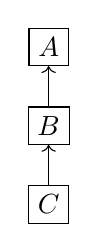
\begin{tikzpicture}
            \node[box] (con) at (0,0) {$A$};
            \node[box] (per1) at (0,-1) {$B$};
            \node[box] (per2) at (0,-2) {$C$};
            \draw[->] (per2) -> (per1);
            \draw[->] (per1) -> (con);
        \end{tikzpicture}
        \figsentence{$A$ because $B$ because $C$.}
        \caption{Chained support}
        \label{fig:chained}
    \end{subfigure}
    \caption{Conjunctions}
    \label{fig:conjunctions}
\end{figure}

Arguments can be supported or attacked by multiple claims in three different ways, as shown in \autoref{fig:conjunctions}. First, multiple claims can cooperatively support the conclusion, implying that attacking one of the claims is sufficient to undermine the conclusion. Second, multiple claims can independently support the conclusion, where attacking one premise does not affect the support of the others on the conclusion. Lastly, the supporting premise itself can be supported.

The grammar for supporting and attacking claims is extended to allow a conclusion to be supported or attacked by multiple claims as shown in the diagrams in Figures~\ref{fig:linked}.

\begin{grammar}
<argument> ::= <claim> `because' <minor-claims> % a <~ b+

<argument> ::= <claim> `but' <minor-claims> % a *~ b+

<minor-claims> ::= <minor-claim-list> `and' <minor-claim>
\alt <minor-claim>

<minor-claim-list> ::= <minor-claim-list> `,' <minor-claim>
\alt <minor-claim>
\end{grammar}

\noindent Independent support (\autoref{fig:multiple}) and chained support (\autoref{fig:chained}) can be expressed using multiple sentences.

\subsection{Rules, warrants, generalizations}
Warranted support and attack combines the usage of the major and minor claims.

\begin{figure}[ht!]
    \centering
    \begin{subfigure}[b]{0.3\textwidth}
        \centering
        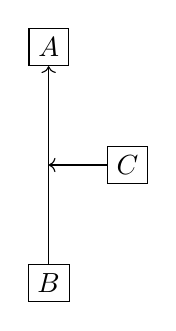
\begin{tikzpicture}
            \node[box] (con) at (0,0) {$A$};
            \node[box] (war) at (1, -1.5) {$C$};
            \node[box] (pre) at (0, -3) {$B$};
            \node[coordinate] (w) at (0, -1.5) {};
            \draw[->] (pre) -- (w) -> (con);
            \draw[->] (war) -> (w);
        \end{tikzpicture}
        \figsentence{$A$ because $B$ and $C_{maj}$.}
        \caption{Warranted support}
        \label{fig:warrantedsupport}
    \end{subfigure}
    \begin{subfigure}[b]{0.3\textwidth}
        \centering
        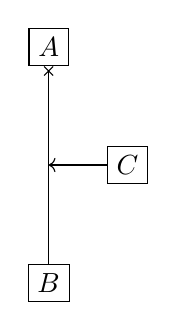
\begin{tikzpicture}
            \node[box] (con) at (0,0) {$A$};
            \node[box] (war) at (1, -1.5) {$C$};
            \node[box] (pre) at (0, -3) {$B$};
            \node[coordinate] (w) at (0, -1.5) {};
            \draw[-x] (pre) -- (w) -> (con);
            \draw[->] (war) -> (w);
        \end{tikzpicture}
        \figsentence{$A$ but $B$ and $C_{maj}$.}
        \caption{Warranted attack}
        \label{fig:warrantedattack}
    \end{subfigure}
    \begin{subfigure}[b]{0.3\textwidth}
        \centering
        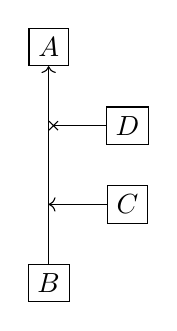
\begin{tikzpicture}
            \node[box] (con) at (0,0) {$A$};
            \node[box] (war) at (1, -2) {$C$};
            \node[box] (pre) at (0, -3) {$B$};
            \node[box] (und) at (1, -1) {$D$};
            \node[coordinate] (u) at (0, -1) {};
            \node[coordinate] (w) at (0, -2) {};
            \draw[->] (pre) -- (w) -- (u) -> (con);
            \draw[->] (war) -> (w);
            \draw[-x] (und) -> (u);
        \end{tikzpicture}
        \figsentence{$A$ because $B$ and $C_{maj}$ but $D$.}
        \caption{Undercutter}
        \label{fig:undercutter}
    \end{subfigure}
    \caption{Support using rules and attack thereof}
\end{figure}

\begin{grammar}
<argument> ::= <claim> `because' <minor-claim-list> `and' <major-claim> % (a <~ b+) <~ c

<argument> ::= <claim> `because' <major-claim> `and' <minor-claims> % (a <~ c+) <~ b

<argument> ::= <claim> `but' <minor-claim-list> `and' <major-claim> % (a *~ b+) <~ c

<argument> ::= <claim> `but' <major-claim> `and' <minor-claims> % (a *~ c+) <~ b
\end{grammar}

\noindent These rules add two relations to the argument: one linked relation from the minor premises supporting or attacking the conclusion, and a relation from the major premise supporting the previous linked relation.

Note that \texttt{minor-claim-list} and \texttt{minor-claims} can also consist of only a single claim. There is no \texttt{major-claim-list} or a way to add multiple major premises to a support relation as we only expect at most one major premise to be relevant per relation.

\paragraph{Undercutter}
We need an extra rule to express the undercutter, as we currently have no way to express an attack on a relation. We allow both major and minor claims as the attacking claim since there is no need to make the distinction.

\begin{grammar}
<argument> ::= <claim> `because' <minor-claim-list> `and' <major-claim> `but' <claim> % (a <~ b+) *~ c

<argument> ::= <claim> `because' <major-claim> `and' <minor-claims> `but' <claim> % (a <~ b+) *~ c
\end{grammar}

\subsection{Collapsed arguments}
The grammar thus far is unambiguous: There is only one way for each of the elements of the argument structure to be expressed. For simple examples it is very effective:

\begin{exe}
    \ex Socrates is mortal because he is a man and men are mortal.
    \ex The object is red because the object appears red but it is illuminated by a red light.
\end{exe}

\noindent Other structures, such as the chaining or arguments (\autoref{fig:chained}) and two arguments attacking each other (\autoref{fig:mutual}) are verbose to express:

\begin{exe}
    \ex\label{ex:hasl0tbw} Tweety can fly because he is a bird. He is a bird because he has wings.
    \ex\label{ex:hasl0tbnottb} Tweety is a bird but Tweety is not a bird. Tweety is not a bird but Tweety is a bird.
\end{exe}

\noindent All argument constructions can be formulated with the grammar that has been presented, but some constructions, such as chained support (\autoref{fig:chained}), are less intuitive to formulate because every sentence can consist of only one argumentative statement.

We extend the grammar to also allow argumentative statements to occur inside sentences. I.e. a conclusion from one statement can be the premise in the next.

In most cases we only allow these argumentative statements, which we call major and minor arguments, at the end of the sentence to make the behaviour of how sentences are interpreted more predictable. Since we need to make a distinction between major and minor claims for the warranted support and attack relations, we also need to inherit this distinction in the argumentative statements. Hence we call them \texttt{minor-argument} and \texttt{major-argument} to reflect that their conclusion is respectively a minor or major claim.

\paragraph{Support}
To limit the ambiguity of how supporting clauses can be interpreted, we only allow the repetition of supported conclusions functioning as a supporting premise to happen at the end of the sentence. Therefore \texttt{minor-arguments} only allows the last claim to be of the argued variety.

\begin{grammar}
<minor-argument> ::= <minor-claim> `because' <minor-arguments> % a! <- b+
    \alt <minor-claim>

<minor-arguments> ::= <minor-claim-list> `and' <minor-argument>
\alt <minor-argument>

<minor-claim-list> ::= <minor-claim-list> `,' <minor-claim>
\alt <minor-claim>
\end{grammar}

\noindent The grammar for major premises is adapted likewise.

\begin{grammar}
<major-argument> ::= <major-claim> `because' <minor-arguments> % a! <~ b+
    \alt <major-claim>
\end{grammar}

\paragraph{Multiple support}
In our grammar thus far we can construct multiple support structures (\autoref{fig:multiple}) by writing multiple sentences and repeating the conclusion. We add the syntax to allow us to leave out the repeated conclusion.

\begin{grammar}
<minor-argument> ::= <minor-claim> <reasons>

<reasons> ::= <reason-list> `and' <reason>

<reason-list> ::= <reason-list> `,' <reason>
\alt <reason>

<reason> ::= `because' <minor-argument>
\end{grammar}

\noindent Note that the difference between sentences with linked support and multiple support is the repetition of `because' in each of the separate reasons.

\paragraph{Attack}
The way attacks are expressed is a little different. To allow for mixing supporting and attacking relations to be expressed in the same sentence, we add variants of \texttt{minor-argument} and \texttt{major-argument} that are attacked. However, in text, `but' often only occurs after `because' and we have little expectation of what premise in the exposition so far it will be attacking. To stay true to this behaviour, we allow the attacked premise to be argued itself, unlike in the grammar for support relations. We also only allow the attack argument to occur as an argument (i.e. a sentence) on its own to limit the number of possible ambiguous but unlikely interpretations. Forming chained attacks (like \autoref{fig:chained}) however is allowed.

\begin{grammar}
<argument> ::= <minor-argument> `but' <argument> % a! *~ b

<argument> ::= <major-argument> `but' <argument> % a! *~ b
\end{grammar}

\noindent The grammar rules that express support and attack relations function the same way as the grammar rules that express a single claim. The conclusion of the argument will function as a premise for the next. At the sentence level it does not matter whether the conclusion an argument is a major or minor claim. We remove this distinction at that level using the following rule:

\begin{grammar}
<argument> ::= <major-argument> | <minor-argument>
\end{grammar}

\paragraph{Mutual attack}
In our grammar we already parse claims with negations in them (the optional \texttt{RB} element in many of the \texttt{major-premise} and \texttt{minor-premise} rules), but we do not use this information yet to automatically create a mutual attack relation (\autoref{fig:mutual}) when these two attack each other.

To allow for this we alter the processing of the \texttt{minor-claim} rules that match negated claims to add the flag \emph{negated=True} to the claim. We then also alter the \texttt{argument} and \texttt{minor-argument} rules that match an attack relation between two minor claims to create two relations (effectively a bidirectional relation) if the claims share the same subject, verb and object but one of them has the negated flag set and the other does not. This allows us to only write one sentence instead of both in example~\ref{ex:mutualsoc}.

\subsection{Anaphora resolution}
Currently the pronouns that occur in the input are copied to the boxes in the argument diagram, but this makes the argument more difficult to understand as the order of the sentence, which we normally use to resolve these anaphora, is no longer present. Furthermore, the grammar to express multiple support or attack relations depend on recognizing the repetition of the conclusion, but if the first occurrence of the conclusion contains a name, and the second a pronoun which is an anaphora for that name, the exact text of both claims is different.

We already identify the names and pronouns in our grammar. We alter the rules for claims to also incorporate information on the entity that occurs in the subject of a claim for the purpose of connecting these entities later on.

The data structure that describes these entities allows them to be described as a name, noun and pronoun. If an entity has been mentioned using both a name and a pronoun in the sentence, the final argument structure will have a data structure that has both these slots filled in.

The anaphora resolution process itself is added to the merging of arguments, which occurs at almost every level in the parse tree since all rules built upon \texttt{major-argument} and \texttt{minor-argument} yield these partial argument structures in which multiple claims can occur. The resulting algorithm is similar to Hobbs' algorithm \cite{hobbs1978}.

\begin{figure}[ht!]
    \centering
    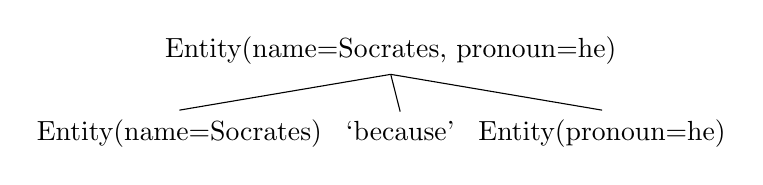
\begin{tikzpicture}
        \Tree [.{Entity(name=Socrates, pronoun=he)} [.{Entity(name=Socrates)} ] `because' [.{Entity(pronoun=he)} ] ]
    \end{tikzpicture}
    \caption{Anaphora resolution inside the parse tree}
    \label{fig:anaphoraresolution}
\end{figure}

The process is redefined as follows:

\begin{enumerate}
    \item All claims from both arguments to be merged are added to the list as a pair consisting of the premise id and the premise itself.
    \item All entities occurring in the claims are extracted from this list and added to a similar list, with pairs of their id and the entity itself.
    \item This list with entities is sorted on the position where the entity first occurred in the input text.
    \item For each entity in the list it is compared to all the following entities to check whether that entity could be referring to it.
    \item If so, the entities are merged, the new merged entity is added to the table, and all occurrences of the two merged entities is replaced with the new entity.
    \item All claims are updated to refer to the new entities using the entity replacement list that has just been constructed. These updated claims are also added to the list with id-claim pairs.
    \item Each claim that occurs multiple times in the list is then replaced with the first occurrence of it in the list. The test to determine whether two claims are the same depend on the updated entities.
    \item The list is used to replace all occurrences of the replaced claims with their replacement in the relations.
    \item The resulting set of unique claims and up-to-date relations is used to create a new argument, the result which is yielded after finishing the grammar rule.
\end{enumerate}

\noindent To determine whether an entity refers to another entity and therefore should be merged, the matching rules in \autoref{table:anaphoraresolution} are used. On the left we have the initial entity. On the top we have the possibly referring entity (which occurred later in the text).

\begin{table}
    \begin{tabular}{r|ccc|}
                & name  & noun  & pronoun \\
        \hline
        pronoun &       &       & =  \\
        noun    &       & =     & yes \\
        name    & =     &       & yes \\
        \hline
    \end{tabular}
    \caption{Pronoun resolution lookup table. To determine whether they should be merged we look at the referring entity and move to the first column for which it has a value. The first test in that column that can be applied will determine the result. If none can be applied, the entities will not be merged. In case of a pronoun the entities are only merged if the first-occurring entity has a matching pronoun or no pronoun at all.}
    \label{table:anaphoraresolution}
\end{table}

In the argument diagram the entities are printed using their most descriptive designation, so preferably their name, then their noun, and otherwise their pronoun. In case of anonymous entities created by the enthymeme resolution process the entities are displayed with the text `something'.

\subsection{Enthymeme resolution}
Parts of the argument are unstated: premises assumed to be known and accepted by all parties are not communicated (or not communicated because they are weak and the speaker does not want to wake sleeping dogs). However, even though these arguments are not part of the argumentative text, they can be supported and attacked by other claims that are. Hence, they have to be drawn in the diagram in order for them to be able to supported or attacked. Therefore we need to reconstruct and draw them.

Enthymemes occur often, and visualising them helps with the understanding of arguments. By doing enthymeme resolution in the same state as the duplication of claims we cannot only fill in the claims that are not stated explicitly, we can also connect the claims that are stated elsewhere in the argument in the right place: the initially missing claim is first reconstructed through the enthymeme resolution process in the place we expect it. If later, when partial arguments higher up in the parse tree are merged and the reconstructed claim is found to be explicitly stated elsewhere in the argument, the reconstructed and original claim are merged.

\paragraph{Rule-like interpretations of claims}
Enthymeme resolution constructs one of the three claims (minor premise, major premise, conclusion) of a syllogism in case the other two are present (\autoref{fig:enthymemes}). To do this we need to interpret the major premises in a different, more rule-like manner.

\begin{exe}
    \ex\label{ex:enthbf} birds can fly
    \ex\label{ex:enthmm} men are mortal
    \ex\label{ex:enthifbf} something can fly if it is a bird
    \ex\label{ex:enthifmm} something is mortal if it is a man
\end{exe}

\noindent We alter the processing of the \texttt{major-claim} rules in the grammar to store them as rules instead of spans of text. For example, examples~\ref{ex:enthbf} and~\ref{ex:enthmm} are how any claim is stored. For the major premise rules we change this to storing them as rules as read in examples~\ref{ex:enthifbf} and~\ref{ex:enthifmm}, replacing the subject with an unspecified entity that occurs as the subject of the major premise and all conditions. This entity functions much like a variable in first-order logic. The original subject is now reformed as a condition for the claim:

\begin{exe}
    \ex something is a man $\to$ something is mortal
\end{exe}

The data structure for major claims  extends the original claim data structure by adding a slot for \emph{conditions}. These conditions themselves are minor claims, but they are not explicitly drawn in the argument diagram. Instead, they are added to the text in the box of the major claim. We allow multiple conditions to, for example, encode the need for linked support by multiple minors.

We add grammar rules for arguments where one of the three premises is missing. In each of these the other two are used to construct the missing third element of the syllogism, and each of the rules will yield a (partial) argument that has all three elements present.

\begin{figure}[ht!]
    \centering
    \begin{subfigure}[b]{0.3\textwidth}
        \centering
        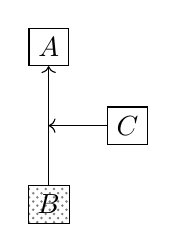
\begin{tikzpicture}
            \node[box] (con) at (0,0) {$A$};
            \node[box] (war) at (1, -1) {$C$};
            \node[box,assumed] (pre) at (0, -2) {$B$};
            \node[coordinate] (w) at (0, -1) {};
            \draw[->] (pre) -- (w) -> (con);
            \draw[->] (war) -> (w);
        \end{tikzpicture}
        \figsentence{$A$ because $C_{maj}$.}
        \caption{Missing minor premise}
        \label{fig:missingminor}
    \end{subfigure}
    \begin{subfigure}[b]{0.3\textwidth}
        \centering
        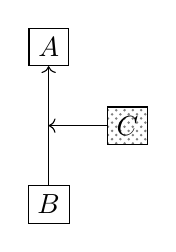
\begin{tikzpicture}
            \node[box] (con) at (0,0) {$A$};
            \node[box,assumed] (war) at (1, -1) {$C$};
            \node[box] (pre) at (0, -2) {$B$};
            \node[coordinate] (w) at (0, -1) {};
            \draw[->] (pre) -- (w) -> (con);
            \draw[->] (war) -> (w);
        \end{tikzpicture}
        \figsentence{$A$ because $B$.}
        \caption{Missing major premise}
        \label{fig:missingmajor}
    \end{subfigure}
    \begin{subfigure}[b]{0.3\textwidth}
        \centering
        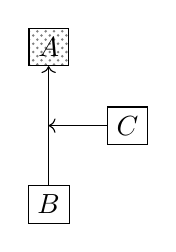
\begin{tikzpicture}
            \node[box,assumed] (con) at (0,0) {$A$};
            \node[box] (war) at (1, -1) {$C$};
            \node[box] (pre) at (0, -2) {$B$};
            \node[coordinate] (w) at (0, -1) {};
            \draw[->] (pre) -- (w) -> (con);
            \draw[->] (war) -> (w);
        \end{tikzpicture}
        \figsentence{$B$ and $C_{maj}$.}
        \caption{Missing conclusion}
        \label{fig:missingconclusion}
    \end{subfigure}
    \caption{Enthymemes originating from syllogisms.}
    \label{fig:enthymemes}
\end{figure}

\paragraph{Missing minor premises}
The missing minor premises are reconstructed from the subject of the conclusion and the conditions of the major premise. For each of the conditions a minor premise is created with the subject of the conclusion and these constructed minor premises are linked to the conclusion using a support relation. This relation is then supported by a support relation originating from the major premise.

\begin{grammar}
<minor-argument> ::= <minor-claim> `because' <major-argument> % (a! <~ ?) <~ b
\end{grammar}

% Given:
%   fly(t) <~ (fly(X) <- bird(X), wings(X))
% Reconstructed:
%   (fly(t) <~ bird(t), wings(t)) <~ (fly(X) <- bird(X), wings(x))

\paragraph{Missing major premise}
The major premise can be reconstructed from the minor premises by creating a condition for each of the minor premises and copying the verb and object from the conclusion to the new major premise.

\begin{grammar}
<minor-argument> ::= <minor-claim> `because' <minor-arguments> % (a! <~ b) <~ ?
\end{grammar}

% Given:
%   fly(t) <~ bird(t), wings(t)
% Reconstructed
%   (fly(t) <~ bird(t), wings(t)) <~ (fly(X) <- bird(X), wings(X))

\paragraph{Missing conclusion}
The conclusion is reconstructed by taking the subject from one of the minor premises and the verb and object from the major premise. We use the subject from the first minor premise as we assume they either all have the same subject or the one most relevant is mentioned first. The constructed major premise is then also the salient premise of this argument.

\begin{grammar}
<minor-argument> ::= <minor-claim-list> `and' <major-argument> % (?! <~ a) <~ b
\end{grammar}

% Given:
%   fly(t) <~ (fly(X) <- bird(X), wings(X))
% Reconstructed
%   (fly(t) <~ bird(t), wings(t)) <~ (fly(X) <- bird(X), wings(X))

\paragraph{Discussion}
Adding recursion will add multiple ways to express the same argument as well as adding multiple ways to interpret argumentative sentences. `a because b but c' can now be interpreted in three ways, but this isn't unexpected..

Major premise data structure is a bit of a missed opportunity. Better would be to have the conditions be part of the argument and define semantics for them so that they can also be added and discussed in the argument itself. Also necessary for Tort.

\section{Evaluation: syllogisms and Toulmin arguments}
We evaluate our implementation by formulating and visualizing different characteristics in arguments --- pros and cons, syllogisms, undercutters --- as well as examples from Toulmin in the context of Toulmin's argument model.

\paragraph{Pros}
Syllogisms always consist of three elements, but not all of them have to be explicitly stated. Example~\ref{evalsyl1} is the complete syllogism, and examples~\ref{evalsylmissingminor},~\ref{evalsylmissingmajor} and~\ref{evalsylmissingconclusion} are the enthymemes.

\begin{exe}
	\ex\label{evalsyl1} Socrates is mortal because he is a man and men are mortal.
	\ex\label{evalsylmissingminor} Socrates is mortal because men are mortal.
	\ex\label{evalsylmissingmajor} Socrates is mortal because he is a man.
	\ex\label{evalsylmissingconclusion} Socrates is a man and men are mortal.
\end{exe}

\noindent \autoref{fig:evalsyl} shows the interpretations. HASL is able to identify the missing premise or conclusion and fill it in. It also correctly identified `he' as a pronoun and instead uses the more descriptive `Socrates' in the boxes.

\begin{figure}[ht!]
    \centering
    \begin{subfigure}[b]{0.3\textwidth}
        \centering
        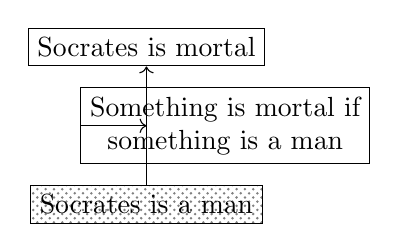
\begin{tikzpicture}
            \node[box] (con) at (0,0) {Socrates is mortal};
            \node[box] (war) at (1, -1) {Something is mortal if\\something is a man};
            \node[box,assumed] (pre) at (0, -2) {Socrates is a man};
            \node[coordinate] (w) at (0, -1) {};
            \draw[->] (pre) -- (w) -> (con);
            \draw[->] (war) -> (w);
        \end{tikzpicture}
        \figsentence{Socrates is mortal because men are mortal.}
        \caption{Missing minor premise}
        \label{fig:evalsylmissingminor}
    \end{subfigure}
    \begin{subfigure}[b]{0.3\textwidth}
        \centering
        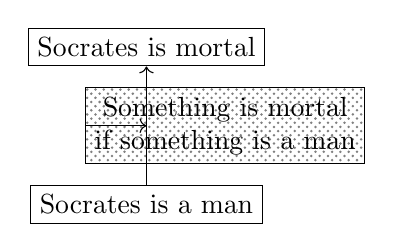
\begin{tikzpicture}
            \node[box] (con) at (0,0) {Socrates is mortal};
            \node[box,assumed] (war) at (1, -1) {Something is mortal\\if something is a man};
            \node[box] (pre) at (0, -2) {Socrates is a man};
            \node[coordinate] (w) at (0, -1) {};
            \draw[->] (pre) -- (w) -> (con);
            \draw[->] (war) -> (w);
        \end{tikzpicture}
        \figsentence{Socrates is mortal because he is a man.}
        \caption{Missing major premise}
        \label{fig:evalsylmissingmajor}
    \end{subfigure}
    \begin{subfigure}[b]{0.3\textwidth}
        \centering
        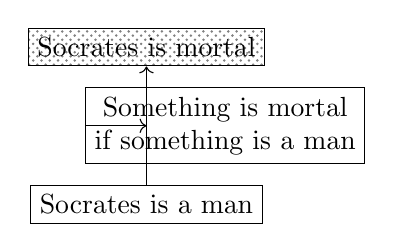
\begin{tikzpicture}
            \node[box,assumed] (con) at (0,0) {Socrates is mortal};
            \node[box] (war) at (1, -1) {Something is mortal\\if something is a man};
            \node[box] (pre) at (0, -2) {Socrates is a man};
            \node[coordinate] (w) at (0, -1) {};
            \draw[->] (pre) -- (w) -> (con);
            \draw[->] (war) -> (w);
        \end{tikzpicture}
        \figsentence{Socrates is a man and men are mortal.}
        \caption{Missing conclusion}
        \label{fig:evalsylmissingconclusion}
    \end{subfigure}
    \caption{Enthymemes originating from syllogisms.}
    \label{fig:evalsyl}
\end{figure}

\paragraph{Cons}
There are many things that can be attacked in an argument. HASL is limited to using keywords and the order of words to identifying what is the claim being attacked.

\begin{exe}
	\ex\label{evalcons1} Tweety can fly because birds can fly but Tweety is a penguin.
	\ex\label{evalcons2} Tweety can fly because Tweety is a bird but Tweety is a penguin.
	\ex\label{evalcons3} Birds can fly but Tweety can not fly because Tweety is a penguin.
\end{exe}

\noindent Examples~\ref{evalcons1} and~\ref{evalcons2} are both interpreted in multiple ways because it is not clear to HASL what is the attacked claim. The first interpretation (\autoref{fig:evalcons1a}) `Tweety is a penguin' is interpreted as an undercutter, while in the second interpretation the claim is interpreted as a direct attack on the major premise (\autoref{fig:evalcons1b}).

The formulation of Example~\ref{evalcons1} is the only way to write an argument with an undercutter, i.e. there needs to be a third claim in the sentence that sets up the relation to attack. There is no way to write an argument with an undercutter without also having additional interpretations.

Which interpretation is the correct interpretation is a discussion topic on its own. Arguably, the interpretation in \autoref{fig:evalcons1a} is ideal because it attacks the argumentation, showing that birds can fly is interpreted as a claim generally assumed to be true but which does allow for exceptions. The second interpretation in \autoref{fig:evalcons1b} shows what happens if the major premise is interpreted as a analytical expression which could be better formulated as `all birds can fly'. The claim that Tweety is a penguin (and therefore Tweety can not fly) is in this case a direct attack on that claim.

Compared to \autoref{fig:evalcons1}, the interpretations in \autoref{fig:evalcons2b} and \autoref{fig:evalcons2c} are new. The interpretation in \autoref{fig:evalcons2b} shows that the grammar in the sentence allows for a nonsensical argument: our definition if penguin excludes this interpretation. If HASL would have had access to such world knowledge these interpretations could be excluded.

\paragraph{Enthymeme resolution}
In \autoref{fig:evalcons1b} the claim that Tweety is a penguin --- and therefore Tweety can not fly --- is in this case a direct attack on that claim. In this interpretation the unstated claim that Tweety can not fly would have been a claim that would have been helpful if drawn, but the enthymeme resolution is only implemented for supporting claims.

In Figures~\ref{fig:evalcons2b} and~\ref{fig:evalcons2c} the unstated major premise is present, but in \autoref{fig:evalcons2a} it is missing. This is a limitation of the grammar: the grammar rule which instantiates the undercutter also has to instantiate the relation to attack, excluding the rules that can instantiate the unstated premise from being applied.

The interpretation in \autoref{fig:evalcons2c} is based on the unstated claim that penguins cannot fly. Having this unstated claim drawn would have been helpful. In \autoref{evalcons3} this is picked up.

When comparing the interpretations of Example~\ref{evalcons1} with Example~\ref{evalcons2} (Figures~\ref{fig:evalcons1} and~\ref{fig:evalcons2}) we observe that assumed claims are never attacked, which is why there is no interpretation equal to \autoref{fig:evalcons1b} in \autoref{fig:evalcons2}, an interpretation that we deemed valid.
 
\begin{figure}[ht!]
	\centering
	\begin{subfigure}[b]{.45\textwidth}
		\centering
		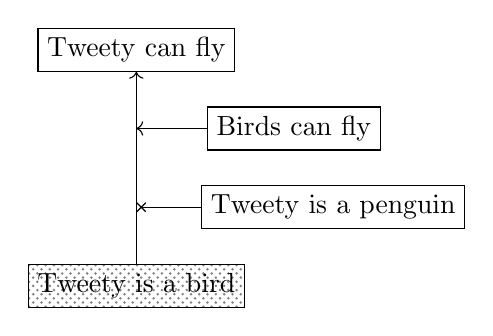
\begin{tikzpicture}
			\node[box] (con) at (0,0) {Tweety can fly};
			\node[box,assumed] (min) at (0,-3) {Tweety is a bird};
			\node[box] (maj) at (2,-1) {Birds can fly};
			\node[box] (und) at (2.5,-2) {Tweety is a penguin};
			\node[coordinate] (smaj) at (0,-1) {};
			\node[coordinate] (sund) at (0,-2) {};
			
			\draw[->] (min) -- (smaj) -| (con);
			\draw[->] (maj) -> (smaj);
			\draw[-x] (und) -> (sund);
		\end{tikzpicture}
		\caption{First interpretation: `Tweety is a penguin' as an undercutter.}
		\label{fig:evalcons1a}
	\end{subfigure}
	\begin{subfigure}[b]{.45\textwidth}
		\centering
		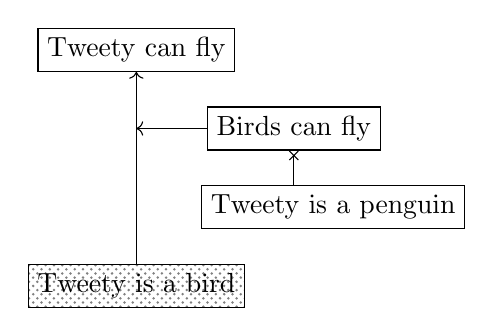
\begin{tikzpicture}
			\node[box] (con) at (0,0) {Tweety can fly};
			\node[box,assumed] (min) at (0,-3) {Tweety is a bird};
			\node[box] (maj) at (2,-1) {Birds can fly};
			\node[box] (att) at (2.5,-2) {Tweety is a penguin};
			\node[coordinate] (smaj) at (0,-1) {};
			
			\draw[->] (min) -- (smaj) -| (con);
			\draw[->] (maj) -> (smaj);
			\draw[-x] (att.north) -| (maj);
		\end{tikzpicture}
		\caption{Second interpretation: `Tweety is a penguin' attacking the major premise.}
		\label{fig:evalcons1b}
	\end{subfigure}
	\figsentence{Tweety can fly because birds can fly but Tweety is a penguin.}
	\caption{Argument diagram for example~\ref{evalcons1}.}
	\label{fig:evalcons1}
\end{figure}

\begin{figure}[ht!]
	\centering
	\begin{subfigure}[b]{.3\textwidth}
		\centering
		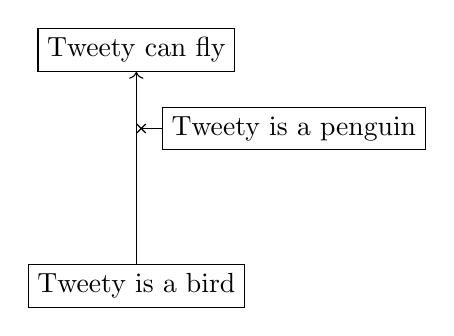
\begin{tikzpicture}
			\node[box] (con) at (0,0) {Tweety can fly};
			\node[box] (min) at (0,-3) {Tweety is a bird};
			\node[box] (maj) at (2,-1) {Tweety is a penguin};
			\node[coordinate] (smaj) at (0,-1) {};
			
			\draw[->] (min) -- (smaj) -| (con);
			\draw[-x] (maj) -> (smaj);
		\end{tikzpicture}
		\caption{First interpretation}
		\label{fig:evalcons2a}
	\end{subfigure}
	\begin{subfigure}[b]{.3\textwidth}
		\centering
		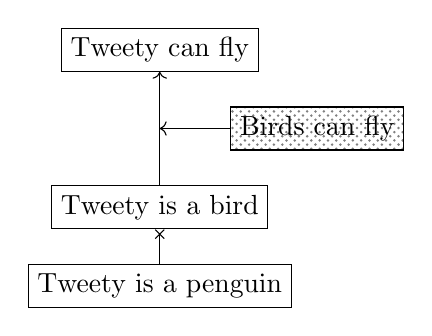
\begin{tikzpicture}
			\node[box] (con) at (0,0) {Tweety can fly};
			\node[box] (min) at (0,-2) {Tweety is a bird};
			\node[box,assumed] (maj) at (2,-1) {Birds can fly};
			\node[box] (att) at (0,-3) {Tweety is a penguin};
			\node[coordinate] (smaj) at (0,-1) {};
			
			\draw[->] (min) -- (smaj) -| (con);
			\draw[->] (maj) -> (smaj);
			\draw[-x] (att) -> (min);
		\end{tikzpicture}
		\caption{Second interpretation}
		\label{fig:evalcons2b}
	\end{subfigure}
	\begin{subfigure}[b]{.3\textwidth}
		\centering
		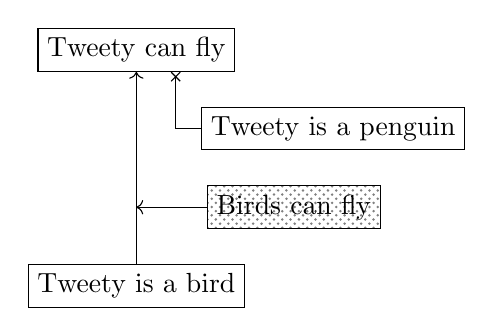
\begin{tikzpicture}
			\node[box] (con) at (0,0) {Tweety can fly};
			\node[box] (min) at (0,-3) {Tweety is a bird};
			\node[box,assumed] (maj) at (2,-2) {Birds can fly};
			\node[box] (att) at (2.5,-1) {Tweety is a penguin};
			\node[coordinate] (smaj) at (0,-2) {};
			
			\draw[->] (min) -- (smaj) -| (con);
			\draw[->] (maj) -> (smaj);
			\draw[-x] (att) -| ([xshift=.5cm]con.south);
		\end{tikzpicture}
		\caption{Third interpretation}
		\label{fig:evalcons2c}
	\end{subfigure}
	\figsentence{Tweety can fly because Tweety is a bird but Tweety is a penguin.}
	\caption{Argument diagram for example~\ref{evalcons2}.}
	\label{fig:evalcons2}
\end{figure}

\begin{figure}[ht!]
	\centering
	\begin{subfigure}[b]{\textwidth}
		\centering
		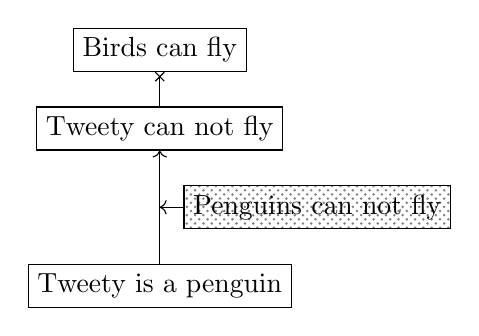
\begin{tikzpicture}
			\node[box] (con) at (0,0) {Birds can fly};
			\node[box] (att) at (0,-1) {Tweety can not fly};
			\node[box] (sup) at (0,-3) {Tweety is a penguin};
			\node[box,assumed] (maj) at (2,-2) {Penguins can not fly};
			\node[coordinate] (smaj) at (0,-2) {};
			
			\draw[-x] (att) -> (con);
			\draw[->] (sup) -- (smaj) -> (att);
			\draw[->] (maj) -> (smaj);
		\end{tikzpicture}
	\end{subfigure}
	\figsentence{Birds can fly but Tweety can not fly because Tweety is a penguin.}
	\caption{Argument diagram for example~\ref{evalcons3}.}
	\label{fig:evalcons3}
\end{figure}

\begin{exe}
	\ex\label{evalcons4} The object is red because the object appears red to me but it is illuminated by a red light.
\end{exe}

\begin{figure}[ht!]
	\centering
	\begin{subfigure}[b]{.45\textwidth}
		\centering
		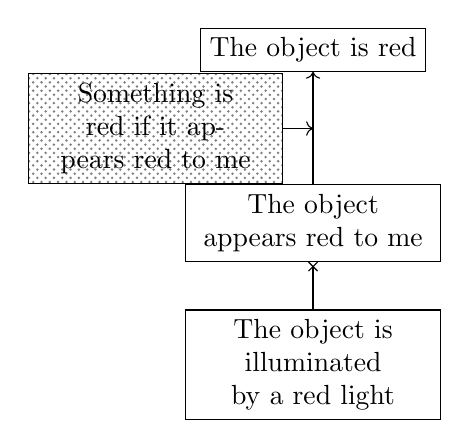
\begin{tikzpicture}
			\node[box] (con) at (0,0) {The object is red};
			\node[box,text width=3cm] (min) at (0,-2.2) {The object appears red to me};
			\node[box,assumed,text width=3cm] (maj) at (-2,-1) {Something is red if it appears red to me};
			\node[box,text width=3cm] (att) at (0, -4) {The object is illuminated by a red light};
			\node[coordinate] (smaj) at (0,-1) {};
			
			\draw[->] (min) -- (smaj) -| (con);
			\draw[-x] (att) -> (min);
			\draw[->] (maj) -> (smaj);
		\end{tikzpicture}
		\caption{First interpretation}
	\end{subfigure}
	\begin{subfigure}[b]{.45\textwidth}
		\centering
		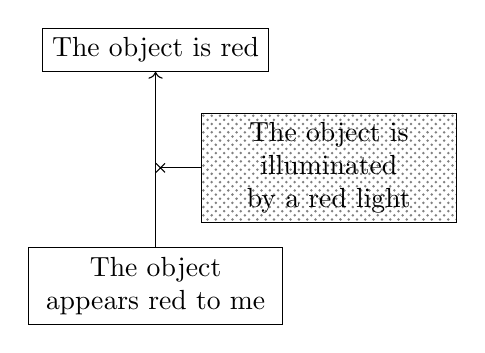
\begin{tikzpicture}
			\node[box] (con) at (0,0) {The object is red};
			\node[box,text width=3cm] (min) at (0,-3) {The object appears red to me};
			\node[box,assumed,text width=3cm] (und) at (2.2,-1.5) {The object is illuminated by a red light};
			\node[coordinate] (sund) at (0,-1.5) {};
			
			\draw[->] (min) -- (sund) -| (con);
			\draw[-x] (und) -> (sund);
		\end{tikzpicture}
		\caption{Second interpretation}
	\end{subfigure}

	\begin{subfigure}[b]{\textwidth}
		\centering
		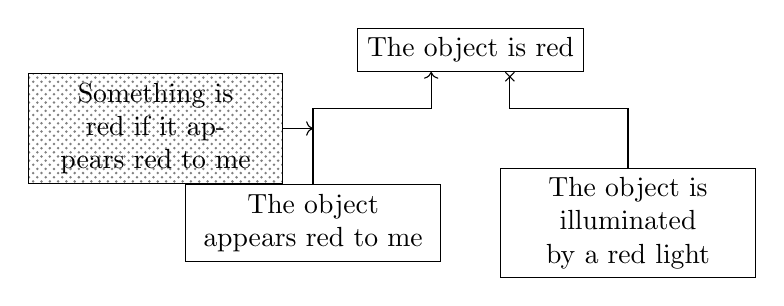
\begin{tikzpicture}
			\node[box] (con) at (0,0) {The object is red};
			\node[box,text width=3cm] (min) at (-2,-2.2) {The object appears red to me};
			\node[box,assumed,text width=3cm] (maj) at (-4,-1) {Something is red if it appears red to me};
			\node[box,text width=3cm] (att) at (2, -2.2) {The object is illuminated by a red light};
			\node[coordinate] (smaj) at (-2,-1) {};
			\node[coordinate] (cmaj) at (-2,-0.75) {};
			\node[coordinate] (catt) at (2,-0.75) {};
			
			\draw[->] (min) -- (smaj) -- (cmaj) -| ([xshift=-0.5cm]con.south);
			\draw[-x] (att.north) -| (catt) -| ([xshift=0.5cm]con.south);
			\draw[->] (maj) -> (smaj);
		\end{tikzpicture}
		\caption{Third interpretation}
	\end{subfigure}
	\figsentence{The object is red because the object appears red to me but it is illuminated by a red light.}
	\caption{Argument diagram for example~\ref{evalcons4}.}
\end{figure}

\paragraph{Toulmin}
Our argument schema can emulate most elements of Toulmin's model. We do not have a specific element for the qualifier of an argument, and our attacks are specifically attacking a claim in the argument as where Toulmin gives attacking arguments their own place in the argument itself.

We formulated two of Toulmin's example arguments, Examples~\ref{ex:harry} and~\ref{ex:petersen}. In the first example we intentionally left out the warrant to test whether this is picked up by HASL. In the second example we do state the warrant (`a Swede can be taken...'), and support it with a backing (`because the portion of...').

\begin{exe}
	\ex\label{ex:harry} Harry is a British subject because Harry is a man born in Bermuda but Harry has become naturalized.
	\ex\label{ex:petersen} Petersen will not be a Roman Catholic because he is a Swede and a Swede can be taken almost certainly not to be a Roman Catholic because the proportion of Roman Catholic Swedes is less than 2\%.
\end{exe}

\noindent Example~\ref{ex:harry} shows the same ambiguity in interpretation we saw in \autoref{fig:evalcons2}: the are three ways to interpret the attack. In two of the three interpretations the warrant is identified, but in the first interpretation it is missing for the reasons described earlier with \autoref{fig:evalcons2a}.

\begin{figure}[ht!]
	\centering
	\begin{subfigure}[b]{\textwidth}
		\centering
		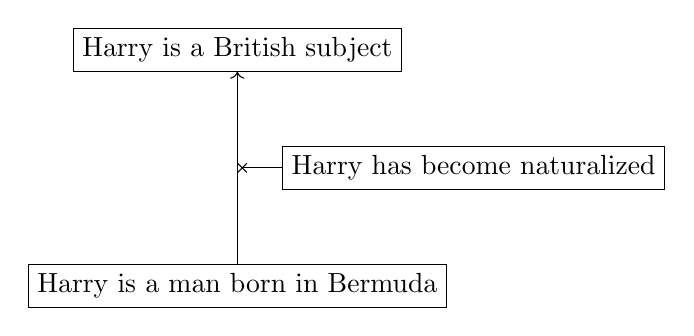
\begin{tikzpicture}
			\node[box] (con) at (0,0) {Harry is a British subject};
			\node[coordinate] (cund) at (0,-1.5) {};
			\node[box] (und) at (3,-1.5) {Harry has become naturalized};
			\node[box] (dat) at (0,-3) {Harry is a man born in Bermuda};
			\draw[->] (dat) -- (cund) -> (con);
			\draw[-x] (und) -> (cund);
		\end{tikzpicture}
		\caption{First interpretation: Being naturalized is an exception to the general rule.}
	\end{subfigure}
	\par\medskip % force a bit of vertical whitespace
	\begin{subfigure}[b]{\textwidth}
		\centering
		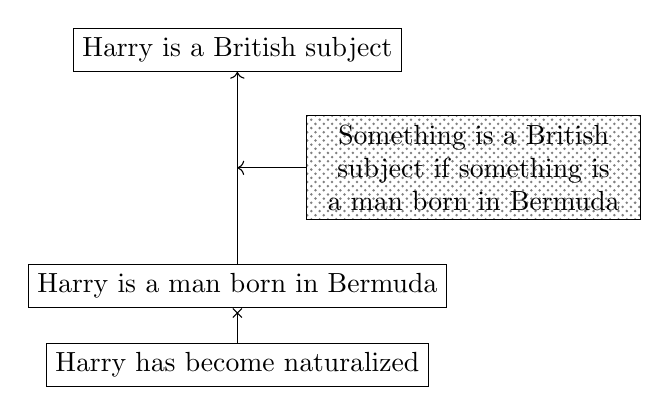
\begin{tikzpicture}
			\node[box] (con) at (0,0) {Harry is a British subject};
			\node[coordinate] (cwar) at (0,-1.5) {};
			\node[box,assumed,text width=4cm] (war) at (3,-1.5) {Something is a British subject if something is a man born in Bermuda};
			\node[box] (dat) at (0,-3) {Harry is a man born in Bermuda};
			\node[box] (att) at (0,-4) {Harry has become naturalized};
			\draw[->] (dat) -- (cwar) -> (con);
			\draw[->] (war) -> (cwar);
			\draw[-x] (att) -> (dat);
		\end{tikzpicture}
		\caption{Second interpretation: Being naturalized is an argument against being born in Bermuda.}
	\end{subfigure}
	\par\medskip % force a bit of vertical whitespace
	\begin{subfigure}[b]{\textwidth}
		\centering
		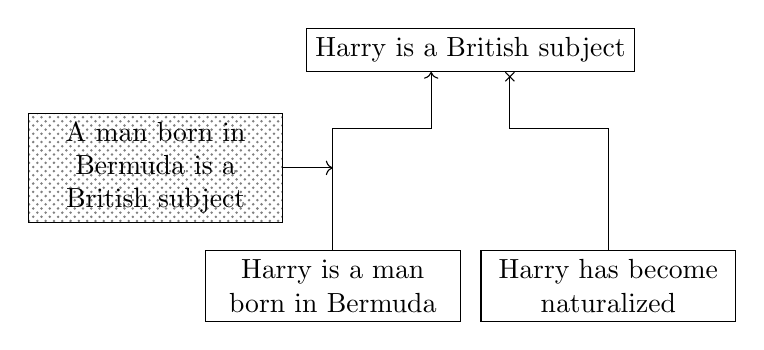
\begin{tikzpicture}
			\node[box] (con) at (0,0) {Harry is a British subject};
			
			\node[box,text width=3cm] (pcon) at (1.75,-3) {Harry has become naturalized}; % datum
			\node[coordinate] (ccon) at (1.75, -1) {}; % budge in (datum -> concl) arrow
			
			\node[box,text width=3cm] (ppro) at (-1.75,-3) {Harry is a man born in Bermuda};
			\node[box,assumed,text width=3cm] (wpro) at (-4,-1.5) {A man born in Bermuda is a British subject};
			\node[coordinate] (spro) at (-1.75, -1.5) {};
			\node[coordinate] (cpro) at (-1.75,-1) {};
			
			\draw[-x] (pcon) -- (ccon) -| ([xshift=.5cm]con.south);
			\draw[->] (ppro) -- (spro) -- (cpro) -| ([xshift=-.5cm]con.south);
			\draw[->] (wpro) -> (spro);
		\end{tikzpicture}
		\caption{Third interpretation: Being naturalized is an argument against being a British subject.}
	\end{subfigure}
	\figsentence{Harry is a British subject because Harry is a man born in Bermuda but Harry has become naturalized.}
	\caption{Argument diagram from HASL/1. Shaded boxes are reconstructed major premises.}
	\label{fig:harry}
\end{figure}

In \autoref{fig:petersen} the interpretations of Example~\ref{ex:petersen} are shown. We have drawn both the interpretations without and with enthymeme resolution to highlight the effect of adding unstated claims to the argument diagram. It shows that although qualifiers are not intentionally taken into account, their meaning is picked up and reflected in the argument.

Furthermore the backing is always correctly placed as supporting the warrant.

\begin{figure}
	\centering
	\begin{subfigure}[b]{\textwidth}
		\centering
		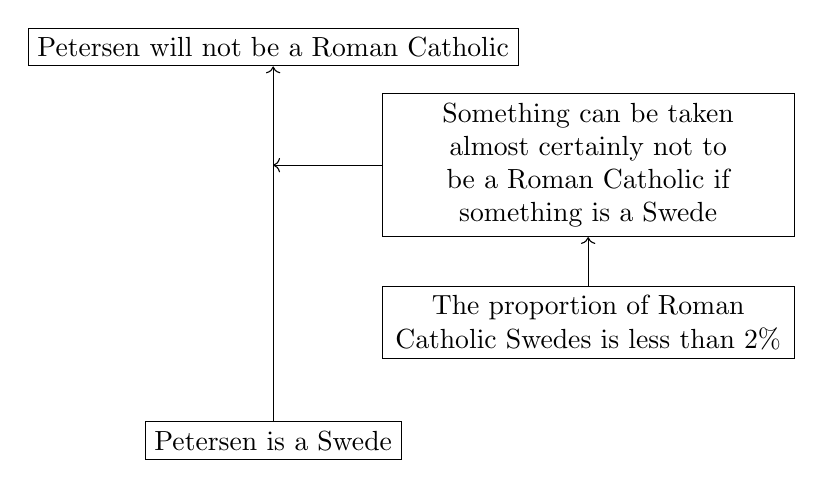
\begin{tikzpicture}
			\node[box] (con) at (0, 0) {Petersen will not be a Roman Catholic};
			\node[box] (sup) at (0, -5) {Petersen is a Swede};
			\node[box,text width=5cm] (maj) at (4, -1.5) {Something can be taken almost certainly not to be a Roman Catholic if something is a Swede};
			\node[box,text width=5cm] (back) at (4, -3.5) {The proportion of Roman Catholic Swedes is less than 2\%};
			\node[coordinate] (smaj) at (0, -1.5) {};
			\draw[->] (sup) -- (smaj) -| (con);
			\draw[->] (maj) -> (smaj);
			\draw[->] (back) -> (maj);
		\end{tikzpicture}
		\caption{Interpretation without enthymeme resolution.}
	\end{subfigure}
	\par\bigskip % force a bit of vertical whitespace
	\begin{subfigure}[b]{\textwidth}
		\centering
		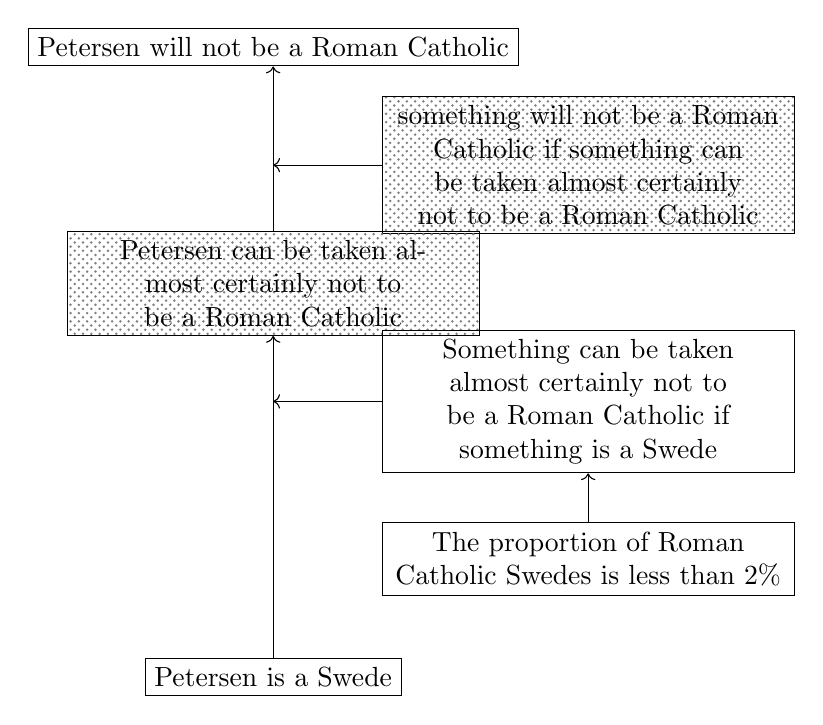
\begin{tikzpicture}
			\node[box] (C1) at (0, 0) {Petersen will not be a Roman Catholic};
			
			\node[coordinate] (X1) at (0, -1.5) {};

			\node[box,text width=5cm,assumed] (B1) at (4, -1.5) {something will not be a Roman Catholic if something can be taken almost certainly not to be a Roman Catholic};

			\node[box,text width=5cm,assumed] (C2) at (0, -3) {Petersen can be taken almost certainly not to be a Roman Catholic};
			
			\node[coordinate] (X2) at (0, -4.5) {};

			\node[box,text width=5cm] (B2) at (4, -4.5) {Something can be taken almost certainly not to be a Roman Catholic if something is a Swede};
			
			\node[box,text width=5cm] (B3) at (4, -6.5) {The proportion of Roman Catholic Swedes is less than 2\%};

			\node[box] (D) at (0, -8) {Petersen is a Swede};

			\draw[->] (C2) -- (X1) -| (C1);
			\draw[->] (B1) -> (X1);
			\draw[->] (D) -- (X2) -| (C2);
			\draw[->] (B2) -> (X2);
			\draw[->] (B3) -> (B2);
		\end{tikzpicture}
		\caption{Interpretation with enthymeme resolution.}
	\end{subfigure}
	\figsentence{Petersen will not be a Roman Catholic because he is a Swede and a Swede can be taken almost certainly not to be a Roman Catholic because the proportion of Roman Catholic Swedes is less than 2\%.}
	\caption{Interpretation of Example~\ref{ex:petersen}.}
	\label{fig:petersen}
\end{figure}

To sum up (yes, this is still mainly for myself as a reminder)
\begin{enumerate}
\item General: Context necessary for ruling out possible targets of the attack.
\item Petersen: Toulmin's backing can be expressed. In a single sentence.
\item Petersen: enthymeme resolution shows the difference between `will not be' and `can be taken almost certainly'.
\item Grammar rules exclude each other. The rule for the undercutter excludes the rule for missing major premise.
\item Enthymeme resolution for attacks would have been really helpful. (in the case of `Tweety can fly but Tweety is a penguin')
\item Enthymeme resolution which allows for assumed claims to be attacked would have been really helpful since this is a natural thing to do (e.g. in a straw man fallacy)
\item All elements of Toulmin's model except for the qualifier can be modelled. Explicitly modelling the qualifier may not always be necessary.
\end{enumerate}




\section{Discussion of related research}
% \section{Arguments for and against claims}

\paragraph{Formal argumentation theory and Toulmin's model}
We defined how we can express cooperative and independent support and attack for claims, and due to the option to composition arguments we can also model chained support as described by Freeman\cite{Freeman:1991ef}. For attacking claims we can model the undermining, undercutting and rebutting arguments defined by Pollock\cite{pollock1987}. Essentially we have all elements to write arguments that include all elements of Toulmin's model\cite{toulmin1958}.

However, we cannot always express which interpretation we want of our textual arguments. For example, sentences in the form of `$A$ because $B$ but $C$' are always interpreted ambiguously. Differentiating between them is only possible when a semantic understanding of the claims is gained, and requires world knowledge and inference, or by adding more explicit markers to our grammar, making the HASL less a human language and more a programming language. 

Furthermore, the interpretation for attacks in sentences such as `$A$ but $B$ because $C$' are odd. For example, take `Tweety is a bird but Tweety cannot fly because Tweety is a penguin'. This would be interpreted as Tweety cannot fly being an argument against Tweety being a bird. Ideally, we would fill in that Tweety is a bird but Tweety cannot fly is really the argument that Tweety is a bird, birds generally can fly, but Tweety is an exception to this general case as Tweety cannot fly. Interpreting attacking arguments is hard, as there are often enthymemes involved.

A more general problem with formal interpretations of argumentation is that one or more aspects becomes lost. For example, in the textual representation there is the choice in which order the supporting arguments and attacking arguments are presented. The language enforces supporting claims before attacking claims at the sentence level, but an argument can consist of multiple sentences, and the order in which the reasoning is presented among those sentences is free. This order is often relevant to how claims are observed, whether they hold or are compromised and retracted in later sentences. In the diagram model there is no sequential order, and there is no way to express whether an attack was accepted as successful or not.

A similar problem occurs with the resolution of enthymemes. By adding the missing elements of enthymemes of arguments to the argument diagram we do change in a sense the interpretation of the argument. Enthymemes may be intentional, and the resulting augmented argument may not be what the original author of the argument intended. The meaning or weight may become distorted, or it may become clear that the incomplete argument was, after being completed, a bad argument \cite{waltonReed2005}.

In a sense, information is lost in our translation from text to an argument diagram.

\paragraph{Rules and generalisations}

We differentiate between general and specific claims by assuming that specific claims always have a very specific subject: a name, a noun preceded by the determiner `the', or a pronoun such as `he'. General claims have subjects such as plural nouns without determiner, or with the  determiner `a'. When such a general claim occurs in the list of claims of a cooperative support, the general claim is drawn as supporting the support relation itself. These general are parsed as claims with conditions, where enthymeme resolution can create specific claims from each of the conditions by replacing `something' with the subject of the conclusion. 

In AIF and tools based on this model, Walton's argument schemes are often used as a description the reasoning behind an argument supporting or attacking a claim. In our model the general claims are part of the argument itself, and they can be argued like any other claim. This allows us to express Toulmin's backing. 

However, the structure for general rules can be more expressive; it can take into account exceptions, but also a logic like the cooperative and independent support relations for the conditions. This way you could express articles of law, like the definition of a tortious act, as a general claim and as such it could be used by enthymeme resolution to express assumptions in arguments.

\paragraph{Argument mining}

Compared to argument mining our implementation of HASL essentially uses the same three tasks described by Lippi et al.\cite{lippi2016argumentation}. Our final step, the prediction on where claims and arguments fit in the larger argument, is given to us almost for free because this structure is hidden in the input. Other approaches need implement an additional mechanism which decides which claims to connect \cite{cohen1987}.

Our approach depends on the ability to completely parse the argumentative text with its grammar: essentially every word has to fall into place. Most approaches do not depend on such a strict use of language, for good reason\cite{mochales2011argumentation,saintDizier2012,lawrenceReed2015}. It cannot be expected that approach can be expanded to encompass all possible argumentative expressions as they occur in the vast amount of written documents. Our approach depends on discourse markers, and although discourse markers are a very strong indicator for argumentative relations, they do not occur often\cite{lawrenceReed2015}.

\paragraph{Argumentation software}
Since our approach requires a completely parsable textual argument, we can use the information this provides, such as the identification of pronouns and the understanding of the structure of general and specific claims, to augment our argument diagram with the missing claims in anaphora. As far as we can tell this is the first approach that provides this level of understanding as a tool. Since it gives all possible interpretations of a textual argument, it can also help identify unexpected ambiguity or help identify the knowledge about the subject that is required to decide which interpretation is the intended one. For example, the intended meaning of `Tweety is a bird but Tweety is a penguin' can only be grasped when the semantic relation between birds and penguins is understood.


\section{Conclusion}
In this paper we presented HASL, our implementation of a human language for structured argumentation. It allows us to express arguments with cooperative and independent supporting relations between claims, with all three types of attacks, and with general and specific claims in text. These texts can then be interpreted and visualized in argument diagrams, providing two different views on the same argument. The text itself may be ambiguous, but such is intentional as human language is ambiguous as well. In such cases all possible interpretations are presented, which helps understand the nature of the ambiguity, giving the writer either the information to remove it, or to make the educated decision to allow it.

\paragraph{Future research}

The interpretation and own semantics of the rule-like nature of generalized claims is first explored in this version of HASL, but is limited in scope. This structure is currently used to fill in the missing conclusion or the missing minor premises in arguments in the form of syllogisms. In the future we want to expand on these semantics, and allow another level of understanding in the resolution of enthymemes.

Lastly, the grammar itself is very closely related to the resulting argument structure. It might be possible to formulate a process in which the argument diagram itself is deconstructed in smaller arguments that fit sentences, and through the use of the grammar rules formulated as a textual argument. Such a process would need to make up for the information that is lost when translating a textual argument into an argument diagram, but like with the enthymeme resolution educated guesses can be tried out and ambiguity can be dealt with by presenting a multitude of formulations, preferring the ones that, when interpreted again, yield the least ambiguous interpretation.

%
%Diagramming tools (Araucaria, Reason!Able, ArguMed)
%
%Text analysis assistants (Araucaria)
%
%Argument mining
%
%Logical languages (with evaluation)
%
%
%\section{Translating natural language arguments to argument diagrams, and back}
%
%Description of how it all works
%
%(Elementary, representative examples)
%
%\section{Toulmin's diagram}
%
%
%\section{Assessment}
%
%Interesting examples
%
%Things that go wrong!



\bibliographystyle{plain}
\bibliography{cumulative}

\end{document}

